\documentclass{beamer}
%
% Choose how your presentation looks.
%
% For more themes, color themes and font themes, see:
% http://deic.uab.es/~iblanes/beamer_gallery/index_by_theme.html
%
\mode<presentation>
{
  \usetheme{default}      % or try Darmstadt, Madrid, Warsaw, ...
  \usecolortheme{default} % or try albatross, beaver, crane, ...
  \usefonttheme{default}  % or try serif, structurebold, ...
  \setbeamertemplate{navigation symbols}{}
  \setbeamertemplate{caption}[numbered]
} 

\usepackage[english]{babel}
\usepackage[utf8x]{inputenc}
\usepackage{multimedia}
\usepackage{listings}
\usepackage[T1]{fontenc}
%\usepackage{media9}
%\usepackage[dvipdfmx]{media9} % only for latex->dvipdfmx
\usepackage{hyperref}

\title[Gnuplot-workshop]{Gnuplot Workshop}
\author{Suhas Gundimeda}
\institute{Purdue University}
\date{2016 October 26th}

\begin{document}

\begin{frame}
  \titlepage
\end{frame}

\section{Possible variety of plots}
\begin{frame}{You can generate any of these... and more}
\only<1>{
\begin{figure}
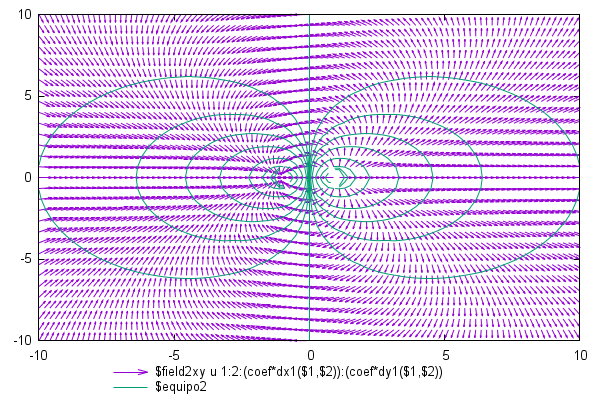
\includegraphics[width=250pt]{vector_3}
\caption{Vector fields}
\end{figure}
}
\only<2>{
\begin{figure}
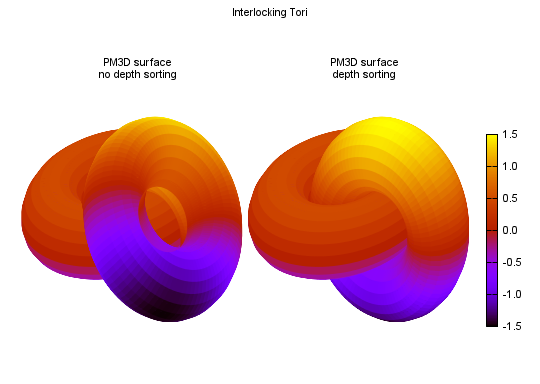
\includegraphics[width=250pt]{tori}
\caption{Interlocking tori}
\end{figure}
}
\only<3>{
\begin{figure}
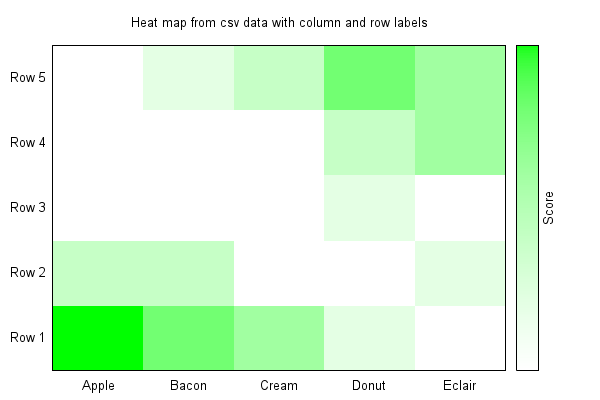
\includegraphics[width=250pt]{heatmap}
\caption{Heatmap}
\end{figure}
}
\note[itemize]{
\item Numerical/calculated plotting (barely touching on this, only the first slide)
\item Experimental plotting}
\end{frame}

\begin{frame}{Outline}
  \tableofcontents
\end{frame}

\section{Why gnuplot?}
\begin{frame}{Why gnuplot?}
\begin{itemize}
\item<1-> Performance
\visible<1>{
\begin{figure}
\includegraphics<1>[width=250pt]{gnuplotperformance}
\caption{Seconds taken to plot 'x' point scatterplot \footnotemark}
\footnotetext{http://stackoverflow.com/a/23883352/1797533}
\end{figure}}
\item<2-> Cross-platform usage
\item<2> Windows, MacOSX, GNU/Linux, BSD, Solaris...
\item<3-> Lots of supported output formats
\item<3> PNG, JPEG, EPS, SVG, DVI, PDF...
\item<4-> One time effort on changing styles $\implies$ personal and consistent plotting.
%\item 4 minutes
\end{itemize}
\end{frame}



\section{Basic 2D function plot}
\begin{frame}{Simple 2D function plot}
\note[itemize]{
\item Walkthrough building a basic graph of a function such as sine.
\item 5 minutes
\item Some modifications and extensions, to get everyone's feet wet on the way things work
\item 10 minutes
}
\end{frame}

%\section{Making it not look like it was generated in the 80s}
%\begin{frame}{Custom styles}
%\note[itemize]{
%\item TODO get a few sets of styles for various uses
%\item Where to put them
%\item 1 minute
%\item Syntax; extending styles
%\item 5 minutes
%\item Where are more styles?
%\item 1 minute
%}
%\end{frame}

\section{Scatter plot}
\begin{frame}{Scatter plot}
\note[itemize]{
\item 4 minutes
}
\end{frame}

\section{Line plot}
\begin{frame}{Connect the dots}
\note[itemize] {
\item 4 minutes
}
\end{frame}

\section{Modifications}
\begin{frame}{Changing axes, legends, colors}
\begin{itemize}
\item Legend: position, titles
\item Axes: ticks, format of numbers, log-scale, arbitrary values
\end{itemize}
\note[itemize] {
\item 5 minutes
\item 10 minutes
\item Colors (lol US spelling)
\item 5 minutes
}
\end{frame}

\begin{frame}{Review}
\note[itemize] {
\item 1 minute
}
\end{frame}

\section{Bar graph}
\begin{frame}{Bar graph}
\note[itemize]{
\item 5 minutes
}
\end{frame}

\section{Miscellaneous}
\begin{frame}{Multiplot layout}
\end{frame}

\begin{frame}[fragile]{gnuplot in \LaTeX}
\begin{lstlisting}
\documentclass{standalone}
\usepackage[miktex]{gnuplottex}
\begin{document}
    \begin{gnuplot}
        set terminal epslatex color  
        set xzeroaxis lt -1
        set yzeroaxis lt -1
        set grid xtics lc rgb '#555555' lw 1 lt 0
        set grid ytics lc rgb '#555555' lw 1 lt 0
        set yrange [-2:2]
        set xrange [-2*pi:2*pi]
        set sample 1000
        plot abs(sin(x))
    \end{gnuplot}
\end{document}
\end{lstlisting}
\end{frame}

\section{3D plotting}
\begin{frame}{Basic 3D plot}
\note[itemize] {
\item 5 minutes
}
\end{frame}

\section{Plotting in polar coordinates}
\begin{frame}{Polar coordinates}
\note[itemize]{
\item The interlocking tori
\item 5 minutes
}
\end{frame}

\begin{frame}{Modifications}
\begin{itemize}
\item Changing viewpoints
\item Effect of surface mesh size
\end{itemize}
\note[itemize] {
\item Changing viewpoints
\item 5 minutes
\item Changing surface mesh size
\item 2 minutes
}
\end{frame}

\section{Further resources}
\begin{frame}{Further help and resources}
\begin{itemize}
\item \href{gnuplot.info}{Official homepage}
\item \href{gnuplotting.org}{Third party site dedicated to gnuplot}
\item \href{http://www.gnuplot.info/help.html}{gnuplot how to get help article}
\item StackExchange network
\item Book: \href{http://www.manning.com
/janert2}{Gnuplot in action}
\item Book: \href{http://www.packtpub.com/gnuplot-visual-guide-with-plotting-software-cookbook/book}{gnuplot cookbook}
\end{itemize}
\end{frame}

\note[itemize] {
\item Total time: 85 minutes
}
\end{document}
